\chapter{Аналитическая часть}

В данном разделе приведено описание объектов сцены, а также анализ существующих алгоритмов для решения поставленных задач, в результате которого будут выбираются наиболее подходящие из них.

\section{Анализ объектов сцены}

Исходя из цели курсовой работы, на сцене должны находиться следующие объекты:

\begin{itemize}
	\item источник света, расположенный на бесконечности. Для задания вектора направления достаточно 2 угла;
	\item камера. Задается положением в пространстве, а также 3 векторами, задающими систему координат камеры;
	\item ландшафт. Задается картой высот, так как одним из параметров генерации является шаг отрисовки. В связи с тем, что одним из параметров генерации является дальность прорисовки, а камера может перемещаться в пространстве, ландшафт должен быть бесконечным. Однако в таком случае его невозможно будет сгенерировать, поэтому вместо этого ландшафт разбивается на множество небольших квадратных участков, чтобы генерировать только в пределах прорисовки. В зависимости от траектории камеры некоторые участки должны генерироваться во время работы программы в произвольный момент времени. 
\end{itemize}

\section{Анализ алгоритмов генерации ландшафта}

\subsection{Алгоритм diamond-square}

Алгоритм diamond-square представляет собой расширенную версию алгоритма midpoint displacement, заключающуюся в использовании двумерной плоскости и наличии 2 этапов \cite{ds}. Первый этап -- <<square>> -- на данном этапе каждый элемент массива -- ромб, для него определяется центральная точка, для которой считается среднее значение из крайних точек и добавляется рандомное смещение. Второй этап -- <<diamond>> -- каждому квадрату в массиве определяется срединная точка, которой устанавливается среднее значение угловых точек и добавляется рандомное смещение. На каждом этапе и при каждой итерации случайное отклонение, которое прибавляется к срединным точкам, уменьшается. На выходе у него получается карта высот, точки в ней расположены по сетке. Таким образом, выходит, что вся плоскость покрыта квадратами. Порядок генерации точек можно увидеть на рисунке \ref{fig:ds}. 

\begin{figure}[h!]
	\centering
	\includegraphics[width=0.6\textwidth]{tex_parts/ds.png}
	\caption{\label{fig:ds}Порядок генерации высот в алгоритме diamond-square \cite{images}}
\end{figure}

 Данный алгоритм хорошо подходит для генерации гор \cite{landscapes}. При этом у данного алгоритма есть сложности с генерацией значений на границах квадрата, так как на шаге square не хватает одной точки. Поэтому в данном случае придётся получать значение по двум точкам, из-за чего границы квадратов могут выделяться. Ещё генератор чисел должен выдавать одинаковые значения для одной и той же точки, в противном случае с одним ключом генерации программа будет генерировать разные ландшафты. Задать порядок генерации чисел не получится, он в любом случае будет зависеть от траектории движения камеры. Также сторона квадрата должна иметь размер $2^n+1$.

\subsection{Fault алгоритм}

Fault  алгоритм  заключаются  в  том,  что  плоскость  разделяется  на  две  части случайной  прямой \cite{fault}.  В  общем  случае,  значения  высот  для  точек,  оказавшихся  с  одной стороны  от  прямой,  понижаются,  а  значения  с  другой стороны повышаются.  Результат алгоритма зависит от количества итераций, которое возможно задать вручную, что продемонстрировано на рисунке \ref{fig:fault}.

\begin{figure}[h!]
	\centering
	\includegraphics[width=0.6\textwidth]{tex_parts/fault.png}
	\caption{\label{fig:fault}Зависимость результата fault алгоритма от количества итераций \cite{images}}
\end{figure}

Для данного алгоритма также потребуется генератор случайных чисел, который будет выбирать точки внутри квадратов в строго определенно порядке в зависимости от ключа генерации и выбранного квадрата. Один из вариантов -- взять генератор случайных чисел от двух точек, значения от которого будут использоваться для создания ключа для генератора чисел для конкретного квадрата, который, в свою очередь, будет использоваться для генерации прямых. Также возникают проблемы со стыковкой соседних квадратов, так как квадраты придётся генерировать независимо друг от друга, и нет никакой гарантии, что на границах высоты совпадут.

\subsection{Шум Перлина}

Шум Перлина -- это тип градиентного шума, разработанный Кеном Перлином в 1983 году \cite{perlin}. Алгоритм имеет множество применений: процедурную генерацию ландшафта, применение псевдослучайных изменений к переменной и помощь в создании текстур изображений. Чаще всего реализуется в двух, трех или четырех измерениях, но может быть определен для любого количества измерений. Для каждой точки возвращает число в диапазоне от 0 до 1. Результат работы представлен на рисунке \ref{fig:perlin}.

\begin{figure}[h!]
	\centering
	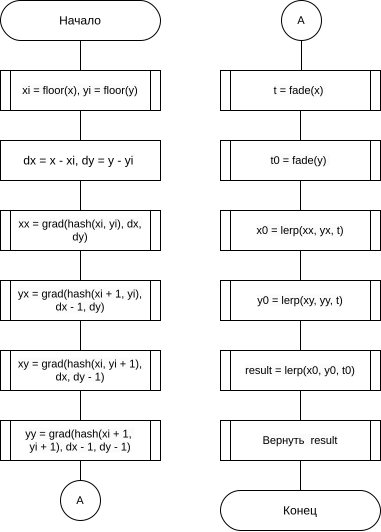
\includegraphics[width=1\textwidth]{tex_parts/perlin.png}
	\caption{\label{fig:perlin}Результат работы алгоритма с использованием шума Перлина \cite{perlin}}
\end{figure}

Данный алгоритм возвращает одно и то же значение для одной координаты при одном ключе генерации вне зависимости от времени вызова, поэтому ландшафт не будет зависеть от траектории движения камеры. кроме того, благодаря данному свойству значения на границах соседних квадратов будут совпадать. Однако при этом алгоритм не подходит для генерации разных классов ландшафтов, но он может использоваться для, например, размывания различных карт высот при комбинировании с другими алгоритмами \cite{landscapes}.

\subsection{Холмовой алгоритм}

Холмовой алгоритм заключается в создании холмов на определенной области \cite{hill}. В зависимости от параметров создаваемых холмов можно создать как скалистую, так и долинистую поверхность. При генерации ландшафт представляется
суперпозицией холмовых функций, где каждый холм образуется полусферой \cite{hill2}. Для достижения реалистичности они иногда генерируются несколькими проходами, высоты холмов на первом проходе соединяются, а карта высот каждого последующего прохода суммируется с картой высот предыдущих. На рисунке ref{fig:hill} показана зависимость результата холмового алгоритма от количества итераций.

\begin{figure}[h!]
	\centering
	\includegraphics[width=0.6\textwidth]{tex_parts/fault.png}
	\caption{\label{fig:hill}Зависимость результата холмового алгоритма от количества итераций \cite{hill}}
\end{figure}

Как и для Fault алгоритма, холмовому алгоритму может потребоваться много итераций для генерации ландшафта. Также в данном случае может потребоваться аналогичная схема с работой генератора случайных чисел. Ещё стоит отметить, что холмы занимают не одну точку на карте и вполне могут попасть на другой квадрат, из-за чего также могут возникнуть проблемы со стыковкой соседних квадратов. 

\subsection{Сравнение алгоритмов}

В таблице \ref{table:landscape} представлены результаты сравнения различных алгоритмов генерации ландшафта. В колонке НГ обозначено отсутствие необходимости в генераторе по 2 числам, в колонке ПС -- отсутствие проблем со стыковкой соседних квадратов, в колонке ННИ -- отсутствие необходимости проводить много итераций.

\begin{table}[h!]
	\small
	\caption{\label{table:landscape}Результаты сравнения алгоритмов генерации ландшафта}
	\begin{center}
		\begin{tabular}{|c|c|c|c|c|}
			\hline
			№ & Название & НГ & ПС & НМИ \\
			\hline
			1 & Diamond-square & {-} & {+} & {+}\\
			\hline
			2 & Fault алгоритм & {-} & {-} & {-}\\
			\hline
			3 & Шум Перлина & {+} & {+} & {+}\\
			\hline
			4 & Холмовой алгоритм & {-} & {-} & {-}\\
			\hline
		\end{tabular}
	\end{center}
\end{table}

В результате сравнения в качестве алгоритмов генерации ландшафта были выбраны алгоритм diamond---square и шум Перлина, так как они способны генерировать бесконечный ландшафт из-за возможности стыковки соседних квадратов.

\section{Анализ алгоритмов удаления невидимых линий и поверхностей}

\subsection{Алгоритм Робертса}

Данный алгоритм работает в объектном пространстве \cite{roberts}.

Сначала идёт подготовка исходных данных. Для каждого тела строится матрица
вида:

\begin{equation}
	\label{eq:D}
	[V] = \begin{bmatrix}
		a_{0} & b_{0} & c_{0} & d_{0} \\
		a_{1} & b_{1} & c_{1} & d_{1} \\
		a_{2} & b_{2} & c_{2} & d_{2} \\
		a_{3} & b_{3} & c_{3} & d_{3} \\
	\end{bmatrix},
\end{equation}

$a, b, c, d$ -- коэффициенты уравнения плоскости грани. Предполагается, что
точки, лежащие внутри тела, дают отрицательное скалярное произведение со всеми уравнениями плоскостей, то есть нормали расположены наружу. Если это не так, то все коэффициенты для уравнения плоскости умножаются на -1.

Следующим шагом является удаление нелицевых граней. Затем происходит удаление ребер, экранируемых другими телами, а также невидимых ребер, образованных линиями пересечения тел, связанных отношениями взаимного протыкания.

Время работы алгоритма $O(N^2)$, где $N$ -- число ребер.

Ландшафт не является выпуклым телом, поэтому для данного алгоритма его придётся изначально разделить на выпуклые тела.

\subsection{Алгоритм Варнока}

Алгоритм Варнока работает в пространстве изображения \cite{varnok} В этом
пространстве рассматривается окно и решается вопрос о том, пусто ли оно
или является его содержимое достаточно простым для визуализации. Если
это не так, то окно разбивается на фрагменты до тех пор, пока содержимое
подокна не станет достаточно просты для визуализации или его размер не
достигнет требуемого предела разрешения. 

Время работы алгоритма $O(CN)$, где $C$ -- количество пикселей в окне, а $N$ -- число полигонов на сцене. В худшем случае придётся рассматривать каждый пиксель как отдельное окно.

\subsection{Алгоритм, использующий Z-буфер}

Алгоритм предложен Эдом Кэтмулом и представляет собой обобщение буфера кадра \cite{algorithms}. Обычный буфер кадра хранит коды цвета для каждого пиксела в пространстве изображения. Идея алгоритма состоит в том, чтобы для каждого пиксела дополнительно хранить еще и координату $Z$ или глубину. При занесении очередного пиксела в буфер кадра значение его $Z$-координаты сравнивается с $Z$-координатой пиксела, который уже находится в буфере. Если $Z$-координата нового пиксела больше, чем координата старого, т.е. он ближе к наблюдателю, то атрибуты нового пиксела и его $Z$-координата заносятся в буфер, если нет, то ни чего не делается. 

Время работы алгоритма $O(CN)$, где $C$ -- количество пикселей в окне, а $N$ -- число полигонов на сцене. 

Одним из главных минусов является высокое потребление памяти за счёт создания Z-буфера.

\subsection{Алгоритм, использующий список приоритетов}

Данный алгоритм иногда называют алгоритмом художника \cite{roberts}. Изначально все полигоны сортируются по глубине или приоритету. Тогда можно записать все элементы в буфер кадра поочередно, начиная с элемента, наиболее удаленного от точки наблюдения. Более близкие к наблюдателю элементы будут <<затирать>> информацию о более далеких элементах в буфере кадра. Эффекты прозрачности можно включить в состав алгоритма путем не полной, а частичной корректировки содержимого буфера кадра с учетом атрибутов прозрачных элементов.

Время работы алгоритма $O(CN)$, где $C$ -- количество пикселей в окне, а $N$ -- число полигонов на сцене. 

Проблема этого алгоритма заключается в том, что иногда приходится отдельно обрабатывать случаи частичного перекрытия интервалов глубины.

\subsection{Алгоритм обратной трассировки лучей}

В данном алгоритме из точки наблюдателя в каждый пиксель экрана выпускается луч \cite{algorithms}. Затем для каждого объекта определяется, пересекается ли он с лучом или нет. Для упрощения вычислений зачастую используют сферическую или прямоугольную оболочку. После этого для пересекающихся объектов вычисляется координата пересечения. В простейшем случае для непрозрачных поверхностей без отражений и преломлений видимой точкой будет точка с максимальным значением $Z$-координаты. Для более сложных случаев требуется сортировка точек пересечения вдоль луча. 

Время работы алгоритма $O(CN)$, где $C$ -- количество пикселей в окне, а $N$ -- число полигонов на сцене. 

Одним из главных минусов является огромное число вычислений, из-за чего он может работать медленнее остальных алгоритмов.

\subsection{Сравнение алгоритмов}

В таблице \ref{table:draw} представлены результаты сравнения алгоритмов удаления невидимых линий и поверхностей. В сложности $C$ обозначает количество пикселей в окне, а $N$ -- число полигонов на сцене.

\begin{table}[h!]
	\small
	\caption{\label{table:draw}Сравнение алгоритмов удаления невидимых линий и поверхностей}
	\begin{center}
		\begin{tabular}{|c|c|c|c|c|}
			\hline
			№ & Название & Пространство & Сложность & Примечание \\
			\hline
			1 & Робертса & Объектное & $O(N^2)$ & \makecell{Работает только\\с выпуклыми объектами} \\
			\hline
			2 & Варнока & Изображения & $O(CN)$ & \makecell{В худшем случае\\придётся рассматривать\\каждый пиксель как окно} \\
			\hline
			3 & Z-буффер & Изображения & $O(CN)$ & \makecell{Потребляет много\\памяти} \\
			\hline
			4 & Художника & Изображения & $O(CN)$ & \makecell{Проблема с перекрывающимися\\интервалами высот} \\
			\hline
			5 & \makecell{Обратной\\трассировки\\лучей} & Изображения & $O(CN)$ & \makecell{Большой объем\\вычислений} \\
			\hline
		\end{tabular}
	\end{center}
\end{table}

В результате сравнения в качестве алгоритма удаления невидимых линий и поверхностей был выбран алгоритм, использующий Z-буффер, так как потребление большего объема памяти наименьшая из проблем в сравнении с другими алгоритмами.

\section{Анализ алгоритмов закраски}

\subsection{Простая закраска}

В данном случае полигон закрашивается полностью одним цветом \cite{algorithms}. Предполагается, что и источник света находится в бесконечности. На изображении могут быть хорошо заметны резкие перепады интенсивности между различно закрашенными многоугольниками, что сильн влияет на реалистичность изображения.

\subsection{Закраска Гуро}

В данном методе нормали в вершинах многоугольников вычисляются как результат усреднения нормалей ко всем полигональным граням, которым принадлежит данная вершина \cite{algorithms}. Далее с помощью билинейной интерполяции вычисляются значения пикселей на сканирующей строке. У данного метода есть недостаток - в результате его применения может появиться эффект полос Маха.

\subsection{Закраска Фонга}

В данном методе значение нормали в вершинах многоугольников вычисляется так же, как и в закраске Гуро \cite{algorithms}. Здесь так же используется билинейная интерполяция для расчета интенсивности в каждом пикселе сканирующей строки, однако вычисляется не сама интенсивность, а вектор нормали в данной точки, с помощью которого уже и вычисляется интенсивность. Данный алгоритм требует больше вычислительных затрат, однако не устраняет эффект полос Маха, хоть и снижает его.

\subsection{Сравнение алгоритмов}

Среди рассмотренных алгоритмов простая закраска наиболее быстрая, так как не требует никаких вычислений, и допустима, так как по условию единственный источник света находится на бесконечности, однако изображение недостаточно реалистично. Поэтому в качестве алгоритма закраски был выбран метод Гуро из-за большей скорости работы в сравнении с методом Фонга.

\section{Выводы}

В данном разделе были формализованы объекты сцены, а также произведён поиск и выбор подходящих алгоритмов для решения поставленной задачи. Для генерации ландшафта было принято решение использовать алгоритм diamond-square и шум Перлина. Для удаления невидимых линий был выбран алгоритм Z-буфера, а для закраски граней -- метод Гуро.